%\documentclass{beamer}
\documentclass[aspectratio=169]{beamer}
\usetheme{Boadilla}

%\usetheme{Warsaw}
%\setbeamercovered{transparent}
\beamertemplatetransparentcoveredhigh
\usepackage[portuges]{babel}
\usepackage[latin1]{inputenc}
\usepackage{lmodern}
\usepackage[T1]{fontenc}
\usepackage{hyperref} 
\usepackage[portuguese, linesnumbered, vlined, titlenumbered, ruled]{algorithm2e}

\newcommand{\eng}[1]{\textsl{#1}}
\newcommand{\cod}[1]{\texttt{#1}}

\title[Apresenta��o]{Curso Intelig�ncia Artificial: do Zero ao Infinito}
\author[Frederico Oliveira]{Evaluation Metrics}
\institute[UFMT]{Universidade Federal de Mato Grosso}
\date{}
%\titlegraphic{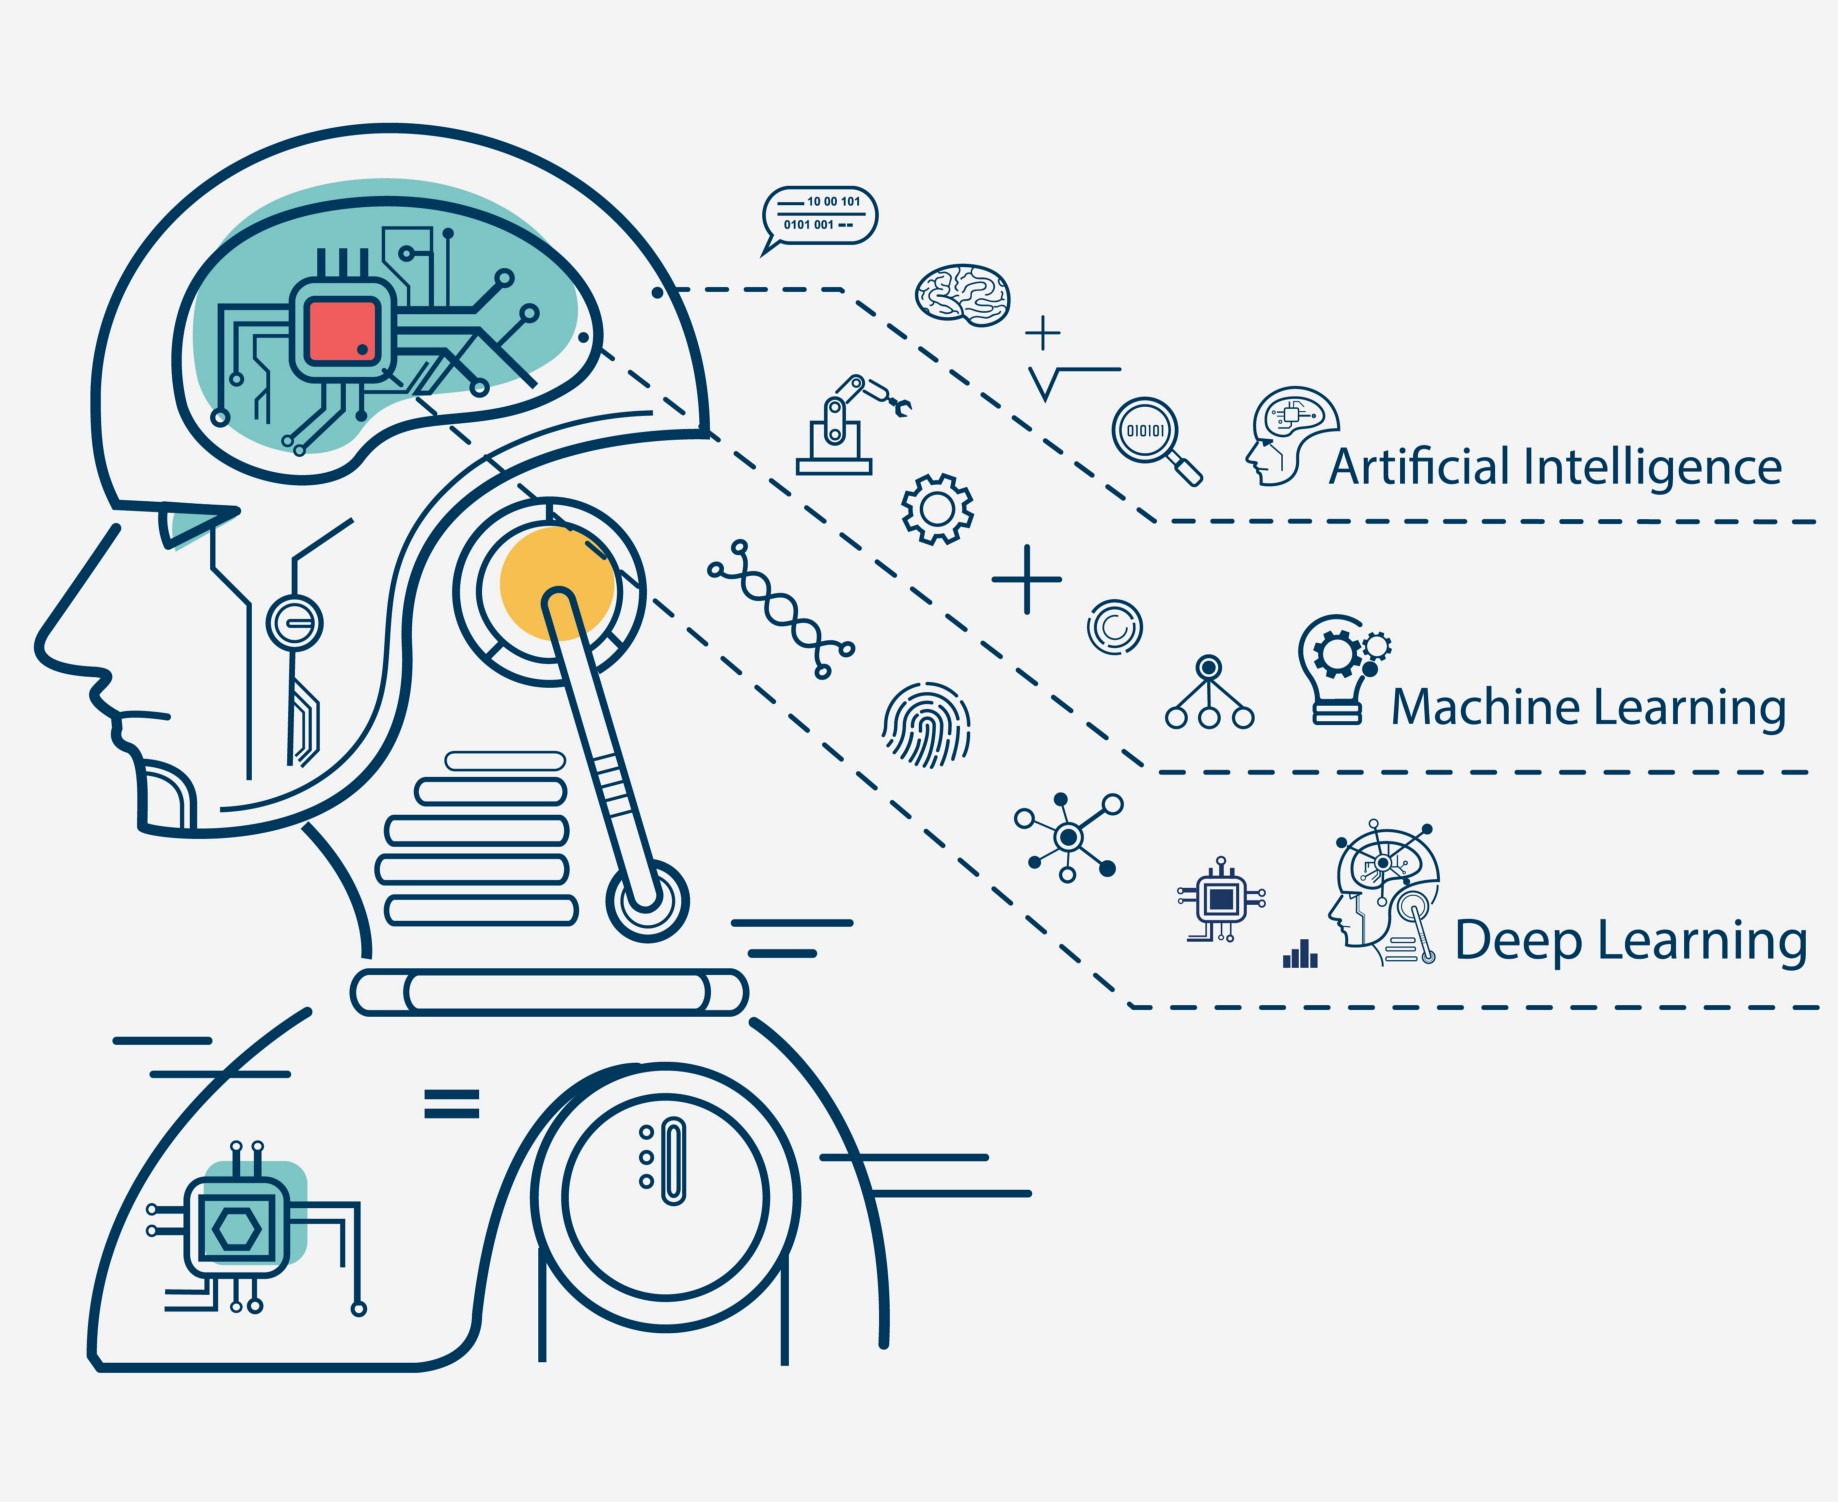
\includegraphics[width=\textwidth,height=.5\textheight]{imgs/intro.jpeg}}
%\usebackgroundtemplate{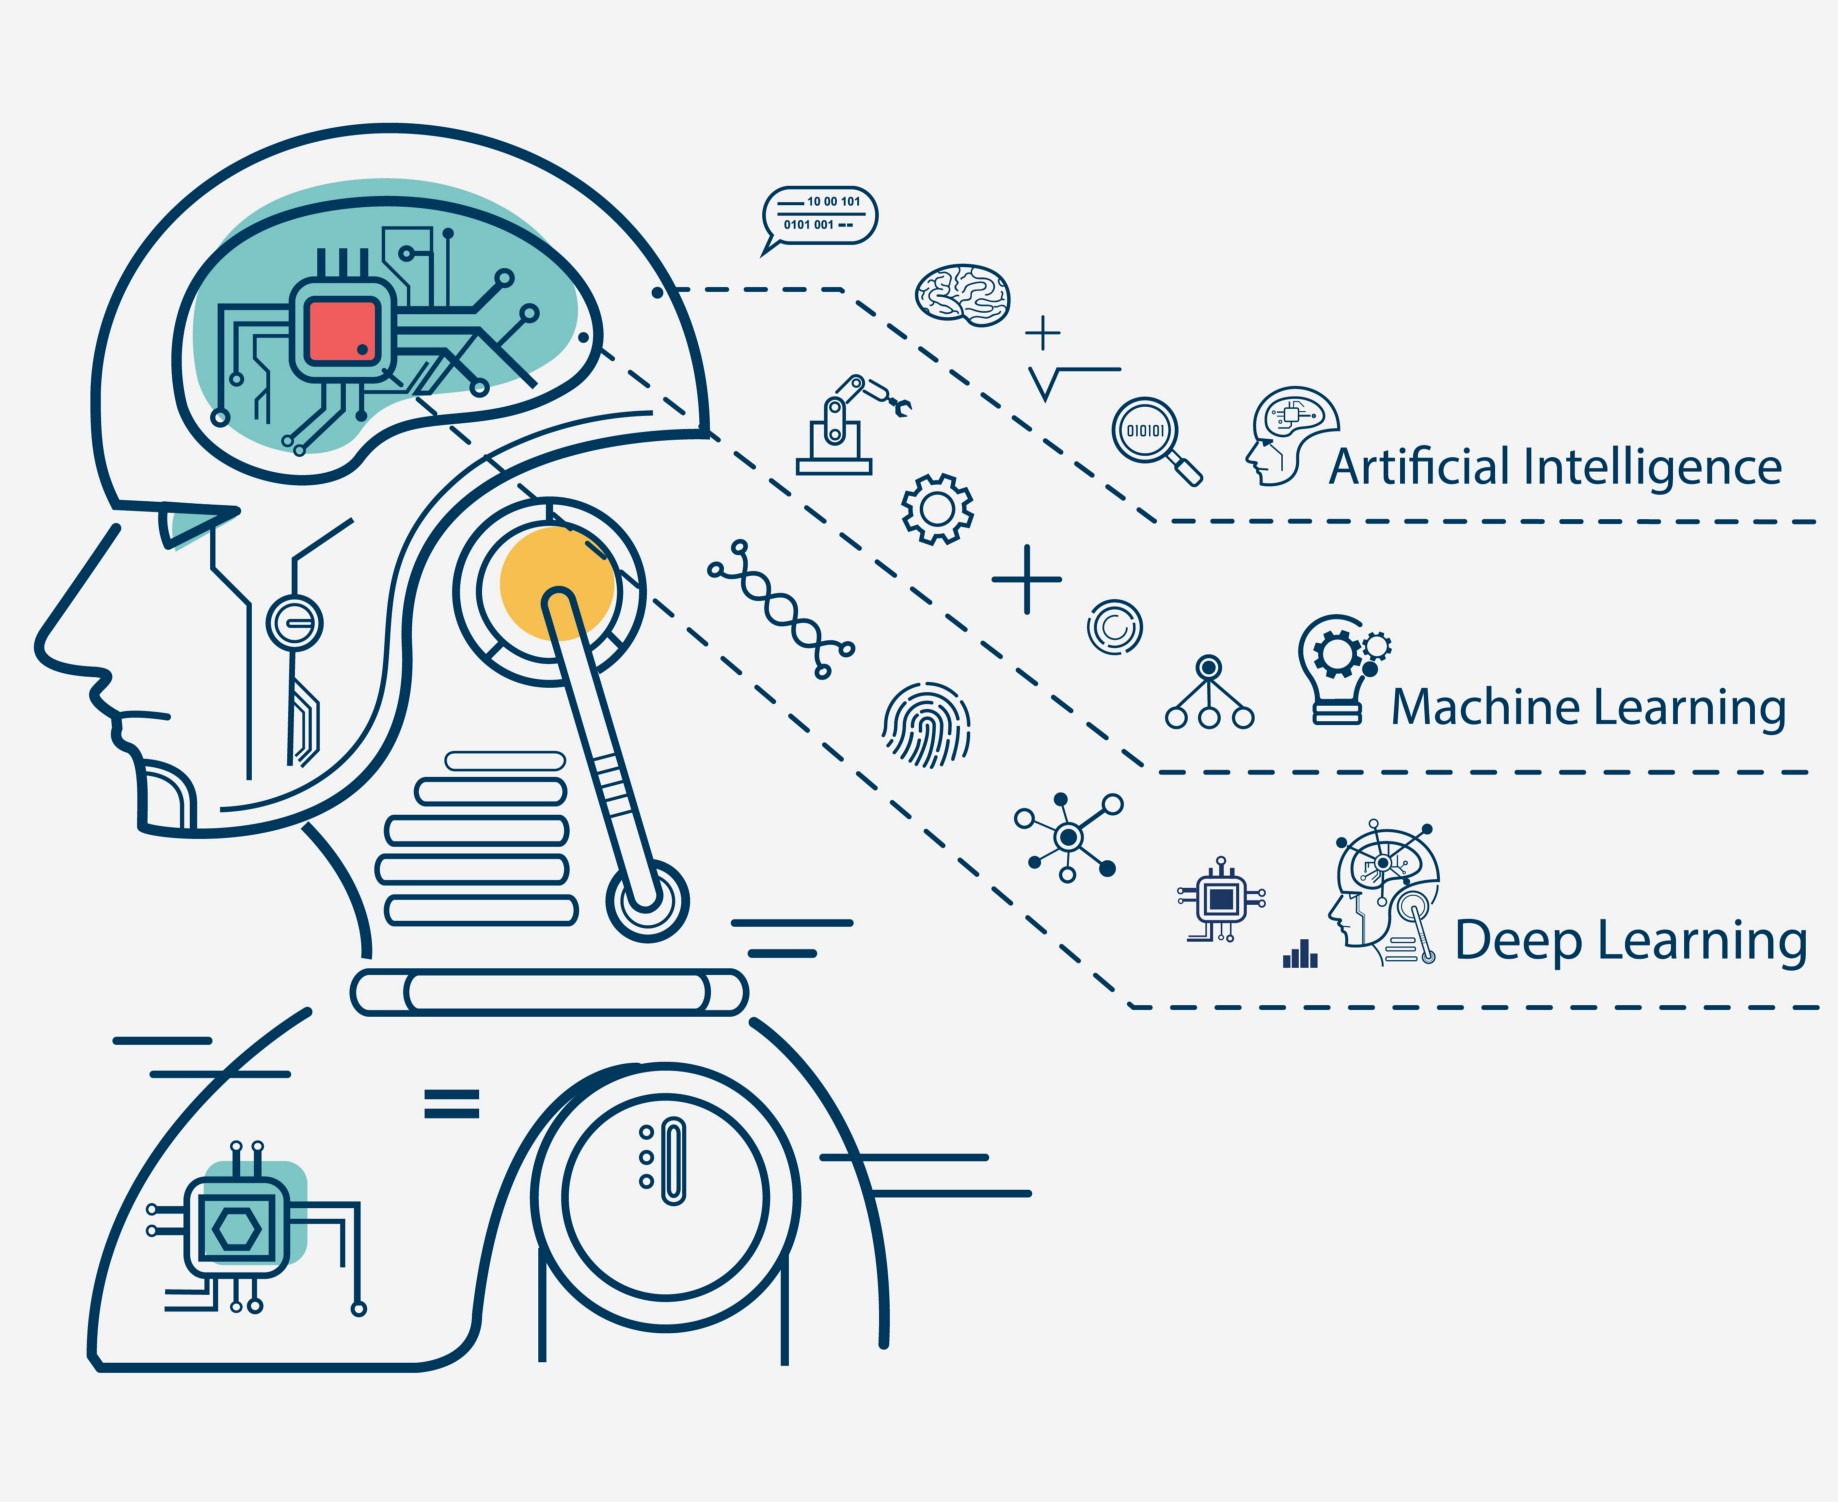
\includegraphics[width=\paperwidth]{imgs/intro.jpeg}}
\begin{document}

\begin{frame}[plain]
  \titlepage
\end{frame}

%%%%%%%%%%%%%%%%%%%%%%%%%%%%%%%%%%%%%%%%%%%%%%%%%%%%%%%%%%%%%%%%%%%%%%%%%%%%%%%%%%%%%%%%%%%%%%%%%%%%%%%%%%%%%%%%
%\section*{Roteiro}
%%%%%%%%%%%%%%%%%%%%%%%%%%%%%%%%%%%%%%%%%%%%%%%%%%%%%%%%%%%%%%%%%%%%%%%%%%%%%%%%%%%%%%%%%%%%%%%%%%%%%%%%%%%%%%%%

\begin{frame}
  \frametitle{Agenda}
  \tableofcontents
\end{frame}



%%%%%%%%%%%%%%%%%%%%%%%%%%%%%%%%%%%%%%%%%%%%%%%%%%%%%%%%%%%%%%%%%%%%%%%%%%%%%%%%%%%%%%%%%%%%%%%%%%%%%%%%%%%%%%%%%
\section{Introduction}
%%%%%%%%%%%%%%%%%%%%%%%%%%%%%%%%%%%%%%%%%%%%%%%%%%%%%%%%%%%%%%%%%%%%%%%%%%%%%%%%%%%%%%%%%%%%%%%%%%%%%%%%%%%%%%%%

\begin{frame}{Introduction}
In object detection, evaluation is non trivial, because there are two distinct tasks to measure:
\begin{itemize}
\item Determining the location of the object (localization, a regression task).
\item Determining whether an object exists in the image (classification)
\end{itemize}

\vspace{1cm}
\tiny{Fonte: \href{https://medium.com/@timothycarlen/understanding-the-map-evaluation-metric-for-object-detection-a07fe6962cf3}{Understanding the mAP Evaluation Metric for Object Detection}}
\end{frame}


%%%%%%%%%%%%%%%%%%%%%%%%%%%%%%%%%%%%%%%%%%%%%%%%%%%%%%%%%%%%%%%%%%%%%%%%%%%%%%%%%%%%%%%%%%%%%%%%%%%%%%%%%%%%%%%%%
\section{Localization}
%%%%%%%%%%%%%%%%%%%%%%%%%%%%%%%%%%%%%%%%%%%%%%%%%%%%%%%%%%%%%%%%%%%%%%%%%%%%%%%%%%%%%%%%%%%%%%%%%%%%%%%%%%%%%%%%

\begin{frame}{Localization}{IoU}
\begin{itemize}
\item In order to evaluate the model on the task of object {\bf localization}, we must first determine how well the model predicted the location of the object.
\item The localization task is typically evaluated on the {\bf Intersection over Union threshold} (IoU).
\end{itemize}

\vspace{1cm}
\tiny{Fonte: \href{https://medium.com/@timothycarlen/understanding-the-map-evaluation-metric-for-object-detection-a07fe6962cf3}{Understanding the mAP Evaluation Metric for Object Detection}}
\end{frame}

%%%%%%%%%%%%%%%%%%%%%%%%%%%%%%%%%%%%%%%%%%%%%%%%%%%%%%%%%%%%%%%%%%%%%%%%%%%%%%%%%%%%%%%%%%%%%%%%%%%%%%%%%%%%%%%%

\begin{frame}{Localization}{IoU}
\begin{itemize}
\item {\bf Intersection over Union} is a ratio between the intersection and the union of the predicted boxes and the ground truth boxes.
\item To get the intersection and union values, we first overlay the prediction boxes over the ground truth boxes. 
\item Now for each class, the area overlapping the prediction box and ground truth box is the intersection area and the total area spanned is the union.
\end{itemize}

\vspace{1cm}
\tiny{Fonte: \href{https://towardsdatascience.com/what-is-map-understanding-the-statistic-of-choice-for-comparing-object-detection-models-1ea4f67a9dbd}{Measuring Object Detection models ? mAP ? What is Mean Average Precision?}}
\end{frame}

%%%%%%%%%%%%%%%%%%%%%%%%%%%%%%%%%%%%%%%%%%%%%%%%%%%%%%%%%%%%%%%%%%%%%%%%%%%%%%%%%%%%%%%%%%%%%%%%%%%%%%%%%%%%%%%%

\begin{frame}{Localization}{IoU}
\begin{figure}[h]
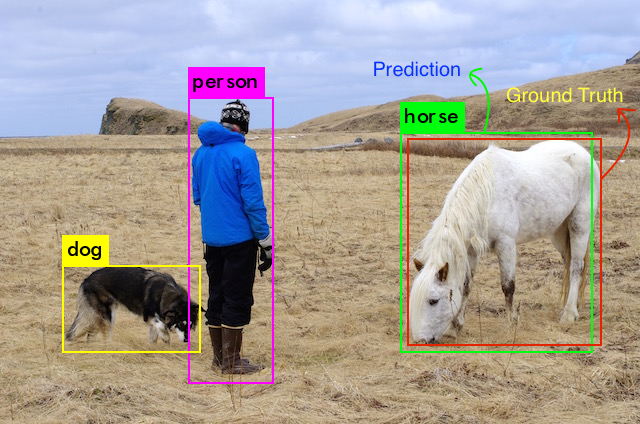
\includegraphics[width=8cm]{imgs/iou_example1.png}
\end{figure}

\end{frame}

%%%%%%%%%%%%%%%%%%%%%%%%%%%%%%%%%%%%%%%%%%%%%%%%%%%%%%%%%%%%%%%%%%%%%%%%%%%%%%%%%%%%%%%%%%%%%%%%%%%%%%%%%%%%%%%%

\begin{frame}{Localization}{IoU}
\begin{figure}[h]
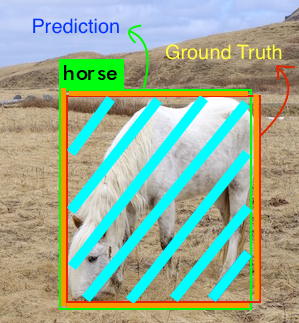
\includegraphics[width=5cm]{imgs/iou_example2.png}
\end{figure}

\end{frame}

%%%%%%%%%%%%%%%%%%%%%%%%%%%%%%%%%%%%%%%%%%%%%%%%%%%%%%%%%%%%%%%%%%%%%%%%%%%%%%%%%%%%%%%%%%%%%%%%%%%%%%%%%%%%%%%%

\begin{frame}{Localization}{IoU}
\begin{figure}[h]
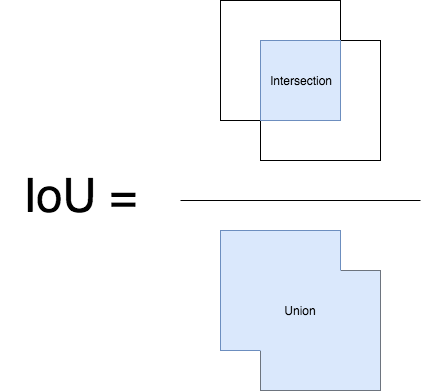
\includegraphics[width=5cm]{imgs/iou.png}
\end{figure}

\end{frame}


%%%%%%%%%%%%%%%%%%%%%%%%%%%%%%%%%%%%%%%%%%%%%%%%%%%%%%%%%%%%%%%%%%%%%%%%%%%%%%%%%%%%%%%%%%%%%%%%%%%%%%%%%%%%%%%%%
\section{Classification}
%%%%%%%%%%%%%%%%%%%%%%%%%%%%%%%%%%%%%%%%%%%%%%%%%%%%%%%%%%%%%%%%%%%%%%%%%%%%%%%%%%%%%%%%%%%%%%%%%%%%%%%%%%%%%%%%

\begin{frame}{Classification}{mAP}
\begin{itemize}
\item In a typical data set there will be many classes and their distribution is non-uniform. 
\item For example there might be many more dogs than cats.
\item There is the need to associate a ''confidence score`` with each bounding box detected and to assess a level of confidence.
\end{itemize}

\vspace{1cm}
\tiny{Fonte: \href{https://medium.com/@timothycarlen/understanding-the-map-evaluation-metric-for-object-detection-a07fe6962cf3}{Understanding the mAP Evaluation Metric for Object Detection}}
\end{frame}

%%%%%%%%%%%%%%%%%%%%%%%%%%%%%%%%%%%%%%%%%%%%%%%%%%%%%%%%%%%%%%%%%%%%%%%%%%%%%%%%%%%%%%%%%%%%%%%%%%%%%%%%%%%%%%%%

\begin{frame}{Classification}{mAP}
\begin{itemize}
\item In order to address these needs, the Average Precision (AP) was introduced. 
\item To understand the AP, it is necessary to understand the {\bf precision} and \bf {recall} of a classifier.
\end{itemize}

\vspace{1cm}
\tiny{Fonte: \href{https://medium.com/@timothycarlen/understanding-the-map-evaluation-metric-for-object-detection-a07fe6962cf3}{Understanding the mAP Evaluation Metric for Object Detection}}
\end{frame}

%%%%%%%%%%%%%%%%%%%%%%%%%%%%%%%%%%%%%%%%%%%%%%%%%%%%%%%%%%%%%%%%%%%%%%%%%%%%%%%%%%%%%%%%%%%%%%%%%%%%%%%%%%%%%%%%
\section{Precision x Recall}
%%%%%%%%%%%%%%%%%%%%%%%%%%%%%%%%%%%%%%%%%%%%%%%%%%%%%%%%%%%%%%%%%%%%%%%%%%%%%%%%%%%%%%%%%%%%%%%%%%%%%%%%%%%%%%%%

\begin{frame}{Precision x Recall}
\begin{figure}[h]
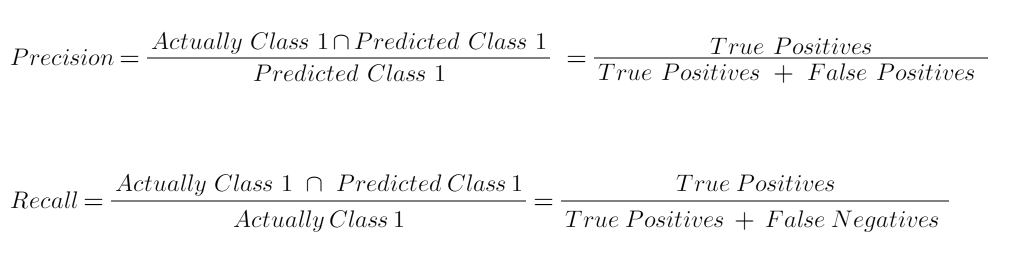
\includegraphics[width=12cm]{imgs/precision_recall.png}
\end{figure}

\vspace{1cm}
\tiny{Fonte: \href{https://analyticsindiamag.com/complete-guide-to-understanding-precision-and-recall-curves/}{Complete Guide to Understanding Precision and Recall Curves}}
\end{frame}

%%%%%%%%%%%%%%%%%%%%%%%%%%%%%%%%%%%%%%%%%%%%%%%%%%%%%%%%%%%%%%%%%%%%%%%%%%%%%%%%%%%%%%%%%%%%%%%%%%%%%%%%%%%%%%%%

\begin{frame}{Precision x Recall}
\begin{figure}[h]
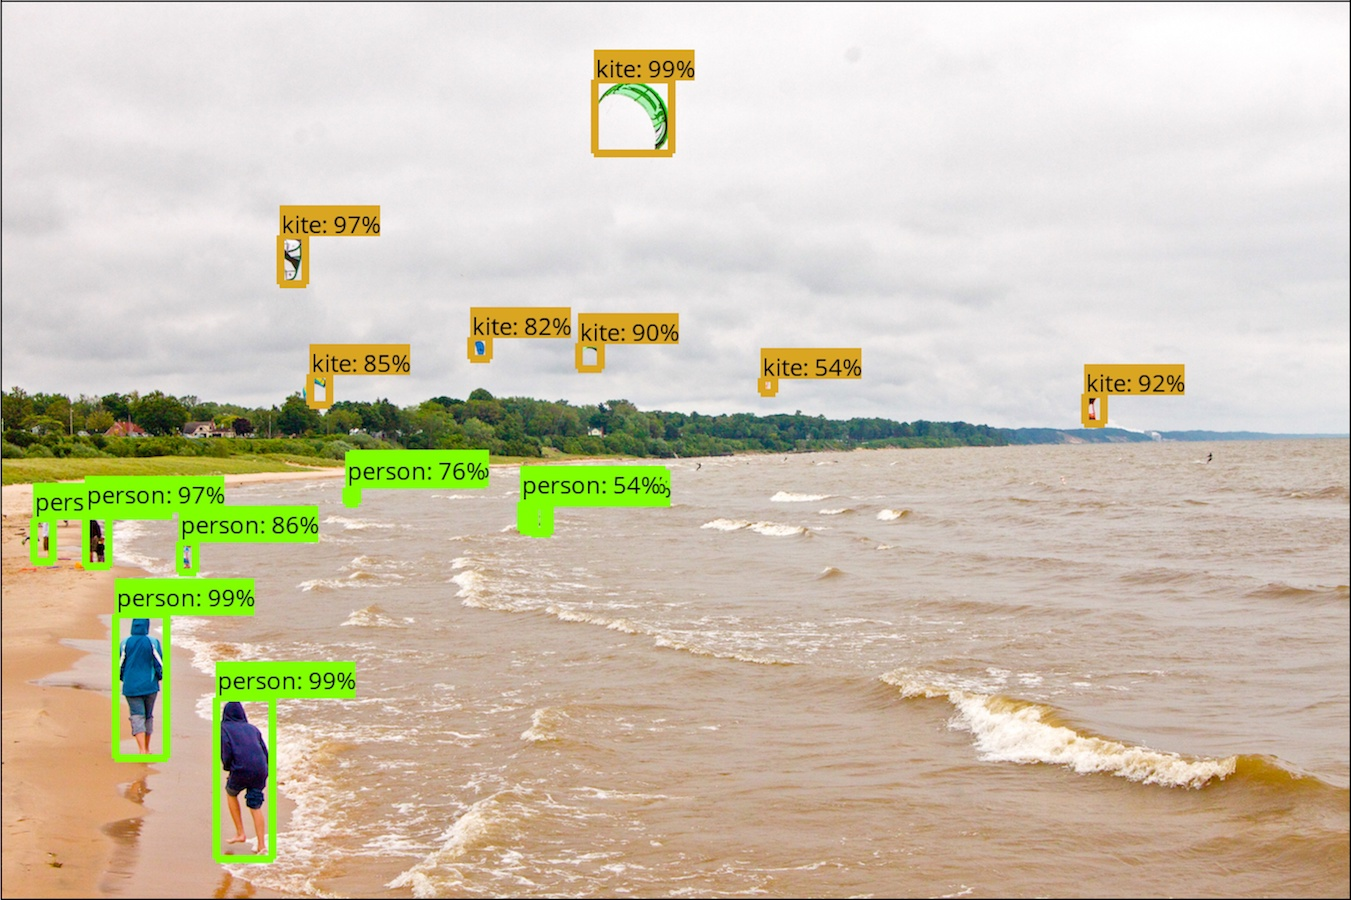
\includegraphics[width=10cm]{imgs/tf_example.jpg}
\end{figure}

\tiny{Fonte: \url{https://github.com/tensorflow/models/tree/master/research/object\_detection\#tensorflow-object-detection-api}}
\end{frame}

%%%%%%%%%%%%%%%%%%%%%%%%%%%%%%%%%%%%%%%%%%%%%%%%%%%%%%%%%%%%%%%%%%%%%%%%%%%%%%%%%%%%%%%%%%%%%%%%%%%%%%%%%%%%%%%%

%\begin{frame}{Precision x Recall}
%\begin{itemize}
%\item Kite, Threshold = 50\%
%\begin{equation}
%P = \frac{7}{7} = 1 = 100%
%R = \frac{7}{7} = 1 = 100%
%\end{equation}
%\item Kite, Threshold = 50\%
%\begin{equation}
%P = \frac{7}{4} = 1 = 100%
%R = \frac{7}{7} = 1 = 100%
%\end{equation}
%\end{itemize}
%\end{frame}

%%%%%%%%%%%%%%%%%%%%%%%%%%%%%%%%%%%%%%%%%%%%%%%%%%%%%%%%%%%%%%%%%%%%%%%%%%%%%%%%%%%%%%%%%%%%%%%%%%%%%%%%%%%%%%%%

\begin{frame}{Precision x Recall}
\begin{figure}[h]
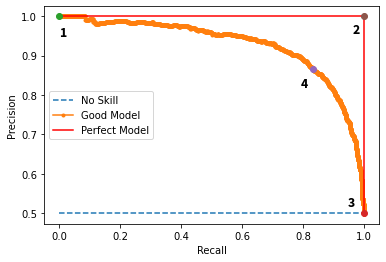
\includegraphics[width=8cm]{imgs/precision_recall_curve.png}
\end{figure}

\tiny{Fonte: \href{https://analyticsindiamag.com/complete-guide-to-understanding-precision-and-recall-curves/}{Complete Guide to Understanding Precision and Recall Curves}}
\end{frame}

%%%%%%%%%%%%%%%%%%%%%%%%%%%%%%%%%%%%%%%%%%%%%%%%%%%%%%%%%%%%%%%%%%%%%%%%%%%%%%%%%%%%%%%%%%%%%%%%%%%%%%%%%%%%%%%%
\section{Mean Average Precision}
%%%%%%%%%%%%%%%%%%%%%%%%%%%%%%%%%%%%%%%%%%%%%%%%%%%%%%%%%%%%%%%%%%%%%%%%%%%%%%%%%%%%%%%%%%%%%%%%%%%%%%%%%%%%%%%%

\begin{frame}{Precision x Recall}
\begin{itemize}
\item The {\bf mean Average Precision} or mAP score is calculated by taking the mean AP over all classes and/or over all IoU thresholds
\end{itemize}
\tiny{Fonte: \href{https://analyticsindiamag.com/complete-guide-to-understanding-precision-and-recall-curves/}{Complete Guide to Understanding Precision and Recall Curves}}
\end{frame}

%%%%%%%%%%%%%%%%%%%%%%%%%%%%%%%%%%%%%%%%%%%%%%%%%%%%%%%%%%%%%%%%%%%%%%%%%%%%%%%%%%%%%%%%%%%%%%%%%%%%%%%%%%%%%%%%

\begin{frame}{Referencias}
\begin{itemize}
\item Measuring Object Detection models ? mAP ? What is Mean Average Precision?
  \begin{itemize}
  \item \url{https://towardsdatascience.com/what-is-map-understanding-the-statistic-of-choice-for-comparing-object-detection-models-1ea4f67a9dbd}
  \end{itemize}
\item Complete Guide to Understanding Precision and Recall Curves
  \begin{itemize}
  \item \url{https://analyticsindiamag.com/complete-guide-to-understanding-precision-and-recall-curves/}
  \end{itemize}  
\end{itemize}
\end{frame}

%%%%%%%%%%%%%%%%%%%%%%%%%%%%%%%%%%%%%%%%%%%%%%%%%%%%%%%%%%%%%%%%%%%%%%%%%%%%%%%%%%%%%%%%%%%%%%%%%%%%%%%%%%%%%%%%

\begin{frame}[plain]
  \titlepage
\end{frame}


\end{document}
